\documentclass[border=10pt]{standalone}
\usepackage{pgfplots}
\pgfplotsset{compat=1.18}
\begin{document}
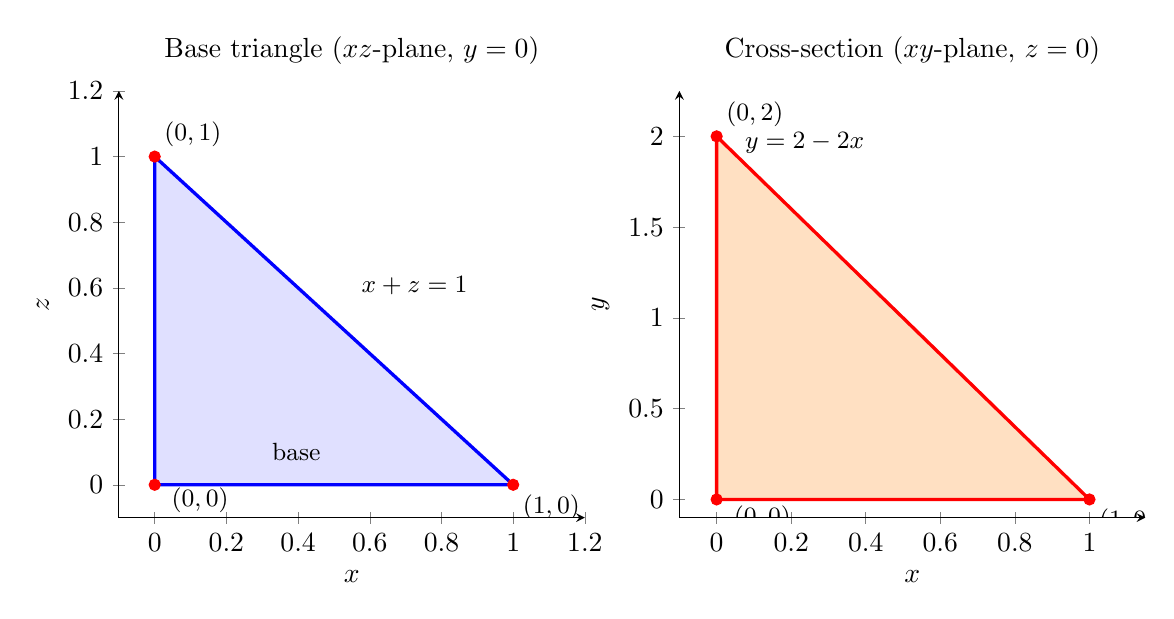
\begin{tikzpicture}
\begin{axis}[
    name=plotL, at={(0,0)}, anchor=south west,
    xlabel={$x$}, ylabel={$z$}, xmin=-0.10, xmax=1.20, ymin=-0.10, ymax=1.20,
    title={Base triangle ($xz$-plane, $y=0$)},
    xtick={0,0.2,...,1.2}, ytick={0,0.2,...,1.2},
    width=7.5cm, height=7cm, axis lines=left, enlargelimits=false,
]
\addplot[fill=blue!20, draw=blue, very thick, fill opacity=0.6] coordinates {
    (0,0) (1,0) (0,1)} -- cycle;
\node[anchor=north west] at (axis cs:0.02,0.02) {\small $(0,0)$};
\node[anchor=north west] at (axis cs:1.0,0)    {\small $(1,0)$};
\node[anchor=south west] at (axis cs:0,1.0)    {\small $(0,1)$};
\node[anchor=south west] at (axis cs:0.55,0.55) {\small $x+z=1$};
\node[anchor=west] at (axis cs:0.30,0.10) {\small base};
\addplot[only marks, mark=*, mark size=2pt, red] coordinates {(0,0) (1,0) (0,1)};
\end{axis}

\begin{axis}[
    name=plotR, at={(plotL.east)}, xshift=1.2cm, anchor=west,
    xlabel={$x$}, ylabel={$y$}, xmin=-0.10, xmax=1.15, ymin=-0.10, ymax=2.25,
    title={Cross-section ($xy$-plane, $z=0$)},
    xtick={0,0.2,...,1.2}, ytick={0,0.5,...,2},
    width=7.5cm, height=7cm, axis lines=left, enlargelimits=false,
]
\addplot[fill=orange!40, draw=red, very thick, fill opacity=0.6] coordinates {
    (0,0) (1,0) (0,2)} -- cycle;
\node[anchor=north west] at (axis cs:0.02,0.02) {\small $(0,0)$};
\node[anchor=north west] at (axis cs:1.0,0)    {\small $(1,0)$};
\node[anchor=south west] at (axis cs:0,2.0)    {\small $(0,2)$};
\node[anchor=south west] at (axis cs:0.05,1.85) {\small $y=2-2x$};
\addplot[only marks, mark=*, mark size=2pt, red] coordinates {(0,0) (1,0) (0,2)};
\end{axis}
\end{tikzpicture}
\end{document}
